\usetikzlibrary{decorations.markings,arrows.meta,bending, patterns}

\subsection*{Page 140, Problem 20 (Worked on all with David LaRoche)}
\vspace{15pt}
\begin{proof}
    \vspace{-10pt}
    \begin{enumerate}[label = (\alph*)]
        \item Split the double torus $T^2$ into the $S^1$ union of two punctured toruses $J, K$ by partitioning a line around its center. Per problem \#109.25, these punctured toruses deformation retract onto the 2-bouquet. This is triangulable because each loop is essentially a triangle complex made of 3 vertices and 3 line segments such that all triangles intersect at a single vertex. Call the loops of $J$ $\langle a,b \rangle$ and the loops of $K$ $\langle c,d \rangle.$ Recall, because no relations exist between generators $a$ and $b$ or $c$ and $d$, that $J$ and $K$ each have fundamental groups equal to the free groups on 2 generators $F_2$.
    
        Next, let's draw our attention to the intersection $S^1 = J \cap K$. This has fundamental group $\Z$ which we can say is generated by some single loop $\langle z \rangle$. Note that the punctured toruses $J, K$ are each equivalent to the square $[0,1]\times[0,1]$ with a circle punched out in the center (and the top/bottom and left/right edges identified with the same direction). $z$ runs around this circle. If we're looking through one side of the partition, without loss of generality, we can let $z$ run clockwise on each such that we can label $a,b,c,d$ in such a way that:
        \begin{center}
            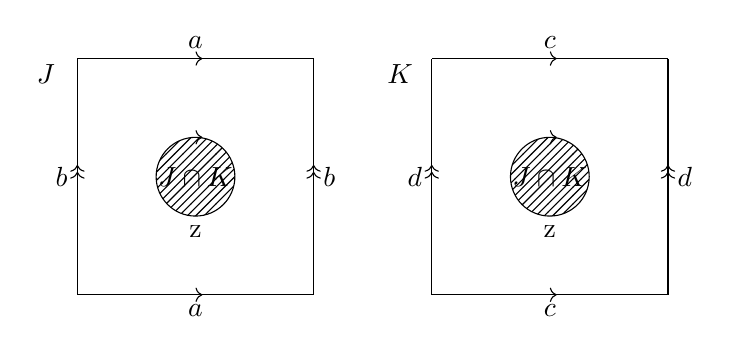
\begin{tikzpicture}
                \tikzset{->-/.style={decoration={
                markings,
                mark=at position #1 with {\arrow{<}}},postaction={decorate}}, ->>-/.style={decoration={
                markings,
                mark=at position #1 with {\arrow{>>}}},postaction={decorate}}}
                
                \draw[->-=.5] (3,0) -- node[below]{$a$} (0,0) ;
                \draw[->-=.5] (3,3) -- node[above]{$a$}(0,3);
                \draw[->>-=.55] (0,0) -- node[left]{$b$} node[xshift=-4mm, yshift = 13mm] {$J$} (0,3);
                \draw[->>-=.55] (3,0) -- node[right]{$b$}(3,3);
                \draw[->-=.25, pattern = north east lines] (1.5,1.5) circle[radius=5mm] node [yshift=-7mm] {z} node {$J \cap K$};

                \begin{scope}[xshift = 4.5cm]
                    \draw[->-=.5] (3,0) -- node[below]{$c$} (0,0) ;
                    \draw[->-=.5] (3,3) -- node[above]{$c$}(0,3);
                    \draw[->>-=.55] (0,0) -- node[left]{$d$}node[xshift=-4mm, yshift = 13mm] {$K$} (0,3);
                    \draw[->>-=.55] (3,0) -- node[right]{$d$}(3,3);
                    \draw[->-=.25, pattern = north east lines] (1.5,1.5) circle[radius=5mm] node [yshift=-7mm] {z} node {$J \cap K$};
                \end{scope}
            \end{tikzpicture}
        \end{center}
    
        Now, finally, because $J, K$ are both triangulable, we can apply Van Kampen's Theorem to some arbitrary basepoint $v$ on $|J \cap K|$ so $$\pi_1(|J\cup K|,v) = \pi_1(|J|,v) *_{\pi_1(|J\cap K,v)}\pi_1(|K|,v).$$ This is equal to the free group of all the generators $a,b,c,d$ along with the `matched' embeddings of relations from the intersection of $J,K$. That is, if we were to homotopy $z$ out until it fit the whole square, the inclusion of $z$ across both generators must match so that, if we start in the bottom left corner and rotate clockwise we get, $j_*(z) = bab^{-1}a^{-1} = dcd^{-1}c^{-1} = k_*(z)$. Because $z$ generates this intersection, this extends to all elements of the fundamental group of the intersection. Simplifying this calculation, we can represent our final group via $$\langle a,b,c,d | bab^{-1}a^{-1}cdc^{-1}d^{-1}=e\rangle.$$

        \item We can perform this calculation a second time with the double torus gluing construction given \href{http://www.map.mpim-bonn.mpg.de/File:Polygon_construction.png}{here}. Now, define $J$ as the entire polygon with a central disc cut out and $K$ as a new disc including $J$'s resected disc which is overlapping some but not fully with $J$. Clearly, $|K|$ will have fundamental group $\{e\}$. Also, $|J\cap K|$ is homotopically equivalent to $S^1$ and thus has fundamental group $\Z$ with generator $z$ rotating, say, clockwise. 
        
        As for $\pi_1(|J|, v)$, we can slowly connect together the tips of $a_1, \bar{a_1}$ and $a_2, \bar{a_2}$, bulging the intermediate single line segments $b_1, b_2$ out until they become loops based at their respective connected tips. Now, identify $a_1, \bar{a_1}$ until it is one segment with its tail at the tails of $\bar{b_1}, \bar{b_2}$ and its tip at the basepoint of loop $b_1$. Now, identify $b_1$ with $\bar{b_1}$ leaving two `finished' loops $a_1, b_1$ at which point we can now identify together $a_2, \bar{a_2}$ so $|J|$ has fully identified to just a 4-bouquet. Per what we did in class, this is triangulable and has fundamental group equal to the free group on 4 generators $a_1,a_2,b_1,b_2$ with no relations.
        
        Now, if we embed our loop $z$ in $|J|$, we can inflate it out until it covers the edges of the polygon. This embedding in $|J|$ gives $j_*(z) = a_1b_1\bar{a_1}^{-1}\bar{b_1}^{-1}a_2b_2\bar{a_2}^{-1}\bar{b_2}^{-1}$. This must match its embedding in $|K|$ which, can also be homotopied all the way down to just the point $\{e\} = k_*(z)$. Therefore, if we retitle $a_1,a_2,b_1,b_2$ as $b,c,a,d$, we get back our previous solution and free product for $v \in |J \cap K|$ of $\pi_1(|J\cup K|, v) = \pi_1(|J|,v) *_{\pi_1(|J\cap K,v)}\pi_1(|K|,v)$ = $$\langle a,b,c,d \mid aba^{-1}b^{-1}cdc^{-1}d^{-1} = e \rangle.$$
    \end{enumerate}
\end{proof}

\subsection*{Page 140, Problem 23}
\vspace{15pt}
\begin{proof}
    \vspace{-10pt}
    Take a path-connected, triangulable space $X$ and disc $D$. The disc is triangulable by the triangle simplex. Note $\pi_1(D) = \{e\}.$ By the formal defintion of an attaching map described on page 71, we can construct a continuous function $f\colon \partial D \to X$ to form the new space $X \cup_f Y$ via an identification map from the boundary circle of $D$ with $X$. Note $\pi_1(X \cap D) = \pi_1(\partial D) = \Z$ has generator $\langle z \rangle$. From here, $z$ has embedding in $D$ that can be shrunk down to just $\{e\}$. And $z$ has some inclusion in $X$ $x_*(z)$. Applying Van Kampen's Theorem to these two triangulable spaces of the disc and $X$ with the path-connected intersection $S^1$, we get that $\pi_1(|X\cup_f D|)$ is the free product that has generators $e$ from the disc and some generators from $X$ with the necessary added relation that the realization $x_*(z)$ and $e$ must be equal. This is an equivalent formulation to quotienting out $\pi_1(|X|)$ by the normal subgroup $N$ of homotopy classes of loops generated by $x_*(z) = e$ so that $$\pi_1(|X\cup_fD|) = \pi_1(|X|)/N.$$ Less abstractly (and rigorously), this attachment is patching up holes in $X$ resulting in loops around those holes being modded out to the identity. 
\end{proof}

\newpage
\subsection*{Page 140, Problem 24}
\vspace{15pt}
\begin{proof}
    \vspace{-10pt}
    Let $G$ be a finitely presented group $\langle g_1, \ldots g_j \mid r_1, r_k \rangle$ with finite generators $g_1, \ldots, g_j$ and finite relations $r_1, \ldots, r_k$, where each $r_i$ is of the form of word $g_i^ag_j^b\cdots g_k^c = e$ (where $i \neq i+1$). Let's start representing a space $X$ with fundamental group $G$ by taking a $j$-bouquet without any relations. This is triangulable as each petal, or loop, of the bouquet is an empty triangle. Also note that each loop represents a generator $g_i$.
    
    To add back the relations from our fundamental group, we will adopt the process explained in problem 23. That is, for each relation $r_i$ of $G$, to add that relation to our bouquet, we can stitch the boundary of a disc along the loops of the bouquet such that the disc boundary will go around the loops in the exact order of the elements of the relation's word and the amount of times as is the integer power of the current element. Attaching a disc for each relation will realize each relation in the bouquet and specifically the modified bouquet's fundamental group.
    
    Next, much aligned with and equally hand-wavy to the idea used in the klein bottle's triangulation, we will avoid any self-intersections in our discs which would make them not triangulable by subdividing the disc's triangle as many times as necessary and stretching or placing the disc in additional dimensions. We can even pull our discs to variegated heights and position them in greater and greater ambient dimensions so they don't intersect.
    
    Thus, the final space will have fundamental group $G$ and be triangulable. It will also be compact because it's closed and bounded in a Euclidean space since the number of discs and dimensions and loops are all finite. But also, according to the attaching description from pages 71-72, the identification space inherits compactness as both the loops and each disc are compact. 
\end{proof}